\documentclass[english]{sobraep}

\title{Visual Question Answering with DeepProbLog}

\author{Jorrit Willaert$^{1}$ \\
	\normalsize $^{1}$Catholic University of Leuven, Leuven -- Belgium \\
	\normalsize e-mail: jorrit.willaert@student.kuleuven.be
}

\begin{document}

\maketitle

\begin{abstract}
	TODO
\end{abstract}

\begin{keywords}
	Neuro Symbolic AI, Visual Question Answering, DeepProbLog, Problog, Convolutional Neural Networks
\end{keywords}

\section{INTRODUCTION}
The Neuro Symbolic AI community is growing rapidly, indicating that people start to recognize the value of the field. The Neuro Symbolic AI field is interested in building a bridge between the robustness of probabilistic knowledge, with the well-known popularity and proven strengths of deep neural networks. DeepProbLog \cite{deepproblog} offers this ability, by using both the strengths of neural networks (i.e. system 1, typical subconscious tasks such as visual recognition, the processing of languages, \dots), along with the strengths of rule-based probabilistic systems (i.e. system 2, slow, sequential thinking such as the derivation of a proof). 

This paper elaborates on an application that requires both systems to be used, namely Visual Question Answering. System 1 will be required in order to gain an understanding of the image under investigation, with in particular their shapes and colors. System 2, on the other hand, will use this extracted information for deriving certain properties of objects\footnote{For example, finding the shape of the green object, or deriving if it is located on the left hand side of the image.}, or even for capturing the relations\footnote{Here, one could think of deriving if an object is located to the left of another object, or also for finding the number of circles in the image.} between the objects. 

\section{ORGANIZATION OF THE PAPER}

\section{LITERATURE SURVEY}
\label{sec:literature_survey}
The application focuses on Visual Question Answering (VQA), for which huge datasets are present, along with very sophisticated methods. The best known dataset for VQA is CLEVR \cite{clevr_dataset}, which contains 100k images with one million questions. An example image is given in Figure \ref{fig:sample_image_clevr}, while example questions are:
\begin{itemize}
    \item Are there an equal number of large things and metal spheres?
    \item What size is the cylinder that is left of the brown metal thing that is left of the big sphere?
    \item How many objects are either small cylinders or metal things?
\end{itemize}

\begin{figure}[H]
    \begin{center}
    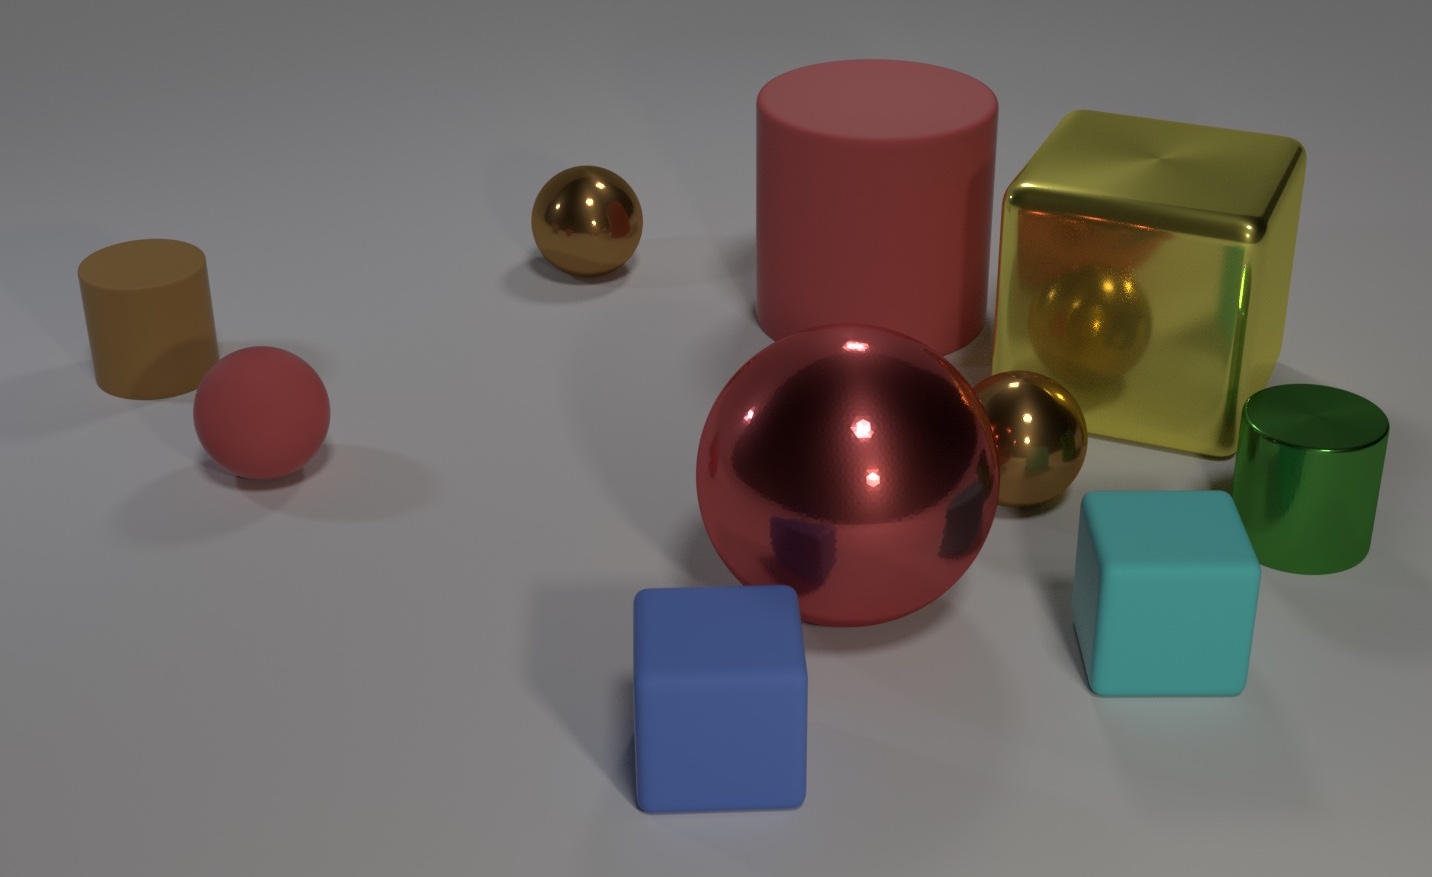
\includegraphics[width=0.3\textwidth]{clevr.jpg}
    \captionsetup{justification=centering}
    \caption{A sample image from the CLEVR dataset \cite{clevr_dataset}}
    \label{fig:sample_image_clevr}
    \end{center}
\end{figure}

Clearly, both system 1 and system 2 are actively used when answering these questions. One could wonder if neural networks alone could answer these questions without having an explicit system 2 encoding (i.e. the rule based knowledge base). Intuitively, it makes sense that if certain facts of the world are known\footnote{They can be encoded, e.g. counting the number of spheres is simply a matter of detecting all the spheres in the image, after which a mathematical summation is a statement in the knowledge base.}, learning can proceed much more quickly\footnote{Not to say that learning might even be impossible if a lot of background knowledge is required.}. Seen from an optimization viewpoint, errors made during prediction in this setup can be targeted exactly, which makes the optimization process also more targeted, and hence more efficient. Finally, this paper also provides evidence for these statements, since in Section \ref{comparison_with_CNN}, the comparison between a VQA implementation with DeepProbLog is made with a purely CNN based approach. % TODO is this the case?

This paper is based on the CLEVR dataset, but uses however a much more simplified version. In essence, it is almost like the Sort-Of-CLEVR dataset \cite{sort_of_clevr_dataset}. This Sort-Of-CLEVR dataset contains images such as in Figure \ref{fig:sample_image_sort_of_clevr}, while asking questions such as:
\begin{itemize}
    \item Non-relational questions: the shape, horizontal or vertical location of an object.
    \item Relational questions: shape of the closest/furthest object to the object under investigation, or the number of objects with the same shape.
\end{itemize}

\begin{figure}[H]
    \begin{center}
    
\includegraphics[width=0.3\textwidth]{sort_of_clevr.png}
    \captionsetup{justification=centering}
    \caption{A sample image from the CLEVR dataset \cite{sort_of_clevr_dataset}}
    \label{fig:sample_image_sort_of_clevr}
    \end{center}
\end{figure}

As explained earlier, both system 1 and system 2 are required for these types of VQA's.

Finally, since this application uses DeepProbLog, quite some time was spent in digesting the DeepProbLog paper \cite{deepproblog}, along with understanding the  examples provided in the code repository \cite{deepproblog_code}.

\section{APPROACH}
The implementation process involved three main parts:
\begin{enumerate}
    \item Generation of data.
    \item Creation of the logical part with DeepProbLog statements.
    \item Linking the data and controlling the training process in pure Python code.
\end{enumerate}

% TODO maybe elaborate why I switched from having a CNN per square in the grid, to one CNN per color.

\subsection{Generation of data}
As mentioned in Section \ref{sec:literature_survey}, the data used in this application is based on the Sort Of CLEVR dataset, with one extra simplification. Given that the logical part will have to decide whether an object is located on the left side of an image, the neural network will have to convey positional information to the logical part. Hence, each discrete position will have to be encoded by a possible outcome of the neural network. Therefore, objects may only be located at certain places in a grid. In this application, a grid of 2x2, 4x4 and 6x6 has been used.

The data generator that was used for the creation of the Sort Of CLEVR dataset has been modified in order to place objects in the mentioned grid positions \cite{sort_of_clevr_dataset}. An example of a generated image is given in Figure \ref{fig:sample_image_own_dataset}.

\begin{figure}[H]
    \begin{center}
    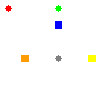
\includegraphics[width=0.3\textwidth]{sample_image_dataset.png}
    \captionsetup{justification=centering}
    \caption{A sample image from the dataset that has been used for this application}
    \label{fig:sample_image_own_dataset}
    \end{center}
\end{figure}

Each specified color will have an object located somewhere in the grid, of which the shape can be a square or a circle.

These images are accompanied with three non-binary questions and one binary question. For each question, a random object is chosen. The possibilities are:
\begin{enumerate}
    \item Non-binary - What is the shape of this object \footnote{I.e. the shape will be either a square or a circle.}?
    \item Non-binary - Is this object located on the left side of the image?
    \item Non-binary - Is this object located on the bottom side of the image?
    \item Binary - How many objects have the same shape of this object?
\end{enumerate}

These questions are encoded in a one-hot encoding, after which they are stored in a CSV file, along with the expected answers. A training set, a validation set, and a test set are generated. % Validation set useful?

\subsection{Controlling the training process}
The overall training process is controlled via the Python interfaces of DeepProbLog, along with general PyTorch implementations of the CNN's.
First of all, CNN's are defined with PyTorch. A relatively simple network is used, where the input is given as a square RGB image of 100 pixels wide, which is transformed by the CNN into 72 output features for the 6x6 grid. Each color that is present in the image has its accompanied CNN network, hence the 72 output features encode the possible positions of the object with that color, along with their shape, which can be either square or circular ($6 \cdot 6 \cdot 2 = 72$).

The final thing (besides the logical rule encodings) required before commencing the training process, are the data loaders. The most challenging part here is the transformation from the generated data to specific query mappings and their outcome. One of the questions are chosen, and a correct mapping between a predicate in the logical rule encoding file and the answer is set up.

\subsection{Logical rule encodings}
Once the CNN belonging to a specific color has determined the position and the shape of that object, logical rules can deduce whether this object is located on the left hand side of the image, on the bottom side, and how many objects have the same shape. The logical rule program has been listed in Appendix \ref{appendix:logical_rule_encodings}

\section{EXPERIMENTS}

\subsection{COMPARISONS WITH PURE SYSTEM 1 APPROACHES}
\label{comparison_with_CNN}
The network based on pure neural predicates is able to recognize the questions quickly, however, seems to experience difficulties when having to decide for the correct answer. This can clearly be seen in the confusion matrix (Figure \ref{fig:confusion_matrix_6x6_pure_NN}). % TODO also talk about confusion matrix of deepproblog

\begin{figure}[H]
    \begin{center}
    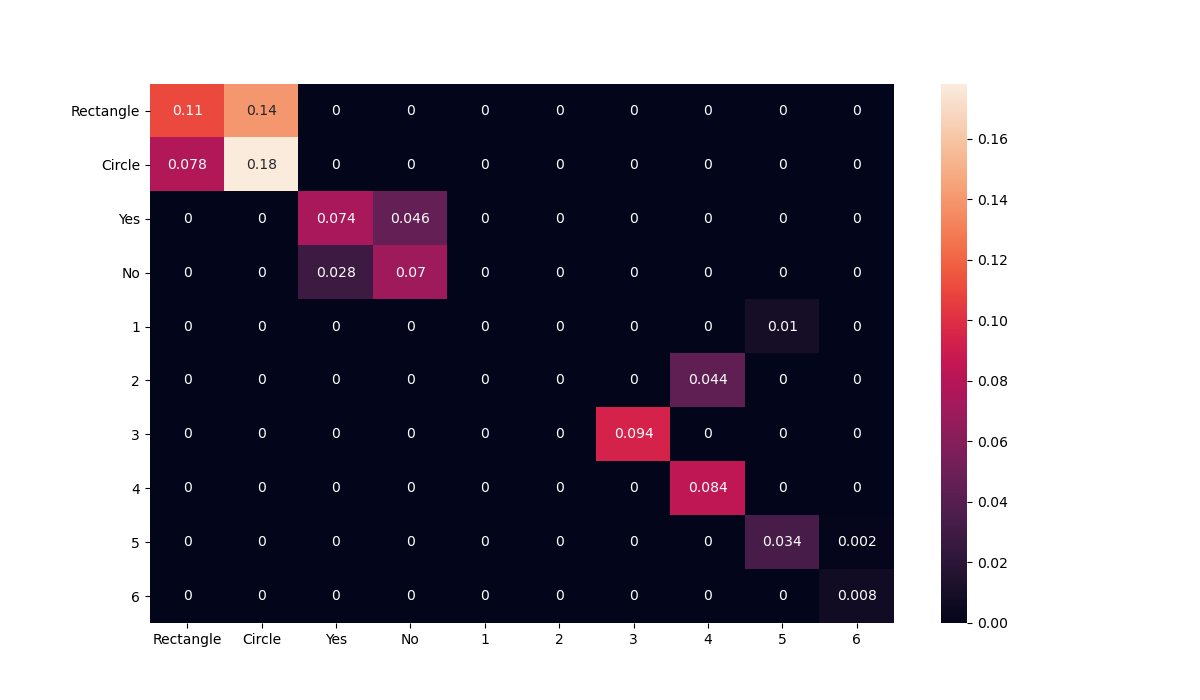
\includegraphics[width=0.3\textwidth]{confusion_matrix_pure_NN_6x6_clear_mistakes.png} 
    \captionsetup{justification=centering}
    \caption{The confusion matrix of the 6x6 dataset on a purely Neural Network based model}
    \label{fig:confusion_matrix_6x6_pure_NN}
    \end{center}
\end{figure}

% Denote difference between epochs and iterations!
% Trained on CPU

It is clear that the network trained with DeepProbLog is able to learn way faster then the purely NN based approach, if measured in the number of iterations \footnote{By the number of iterations, the number of training steps on a batch is meant.}. However, the differences in training time are much less significant% TODO give concrete measures
, due to the high computational cost associated with the arithmetic parts of the circuit (i.e. the semirings).

\section{CONCLUSIONS}


\section{APPENDIX}
\subsection{Logical rule encodings}
\label{appendix:logical_rule_encodings}
% TODO put logical rules here

\bibliographystyle{bib_sobraep}
\bibliography{Capita_Selecta_AI_Initial_Idea} 

%\balance

\end{document}